% !Mode:: "TeX:UTF-8"
% !TEX program= xelatex
\documentclass[a4paper]{article}
\usepackage{amsmath}
\usepackage{amssymb}
\usepackage{ctex}
%\usepackage{fourier}
%\usepackage{braket}
%\usepackage[european]{circuitikz}
\usepackage{multirow}
\usepackage{float}
\usepackage{graphicx}
\usepackage{geometry}
\geometry{left=2.5cm, right=2.5cm, bottom=2.5cm, top=2.5cm}
%\newcommand*{\rom}[1]{\expandafter\@slowromancap\romannumeral #1@}
\newcommand{\rom}[1]{\textup{\uppercase\expandafter{\romannumeral#1}}}
\newcommand{\parallelsum}{\mathbin{\!/\mkern-5mu/\!}}
\title{近代物理实验报告3.5:磁光克尔效应}
\author{xy\quad 学号\quad 匡亚明学院}
\date{2019年2月29日}
\begin{document}
\maketitle
\bibliographystyle{unsrt}
%--------main-body------------

\section{引言}
Michael Farady 首先在 1845 年发现磁光现象,他发现通过玻璃样品的透射
光的偏振面在玻璃样品加上磁场后发生了旋转,这就是现在所知的法拉第效应。
32 年后,John Kerr 发现,从抛光的电磁铁磁极上反射回来的偏振光的偏振面同
样发生了旋转,这就是 magneto-optic Kerr effect。在 1985 年,Moog 和 Bader 首
先将 magneto-optic Kerr effect 应用到表面磁性的研究当中,并称之为表面磁光克
尔效应(SMOKE)。它是指铁磁性样品(如铁、钴、镍及其合金)的磁化状态对
于从其表面反射的光的偏振状态的影响。当入射光为线偏振光时,样品的磁性会
引起反射光偏振面的旋转和椭偏率的变化。
\section{实验目的}
\begin{enumerate}
	\item 了解表面磁光克尔效应的原理和实验方法
\end{enumerate}

\section{实验仪器}
亥姆霍兹线圈、电磁铁、特斯拉计、毫特斯拉计、大功率恒流电源、大功率扫描电源、精密恒流源、数字微伏表、四探针样品夹具。

\section{实验原理}
\begin{figure}[!h]
    \centering
    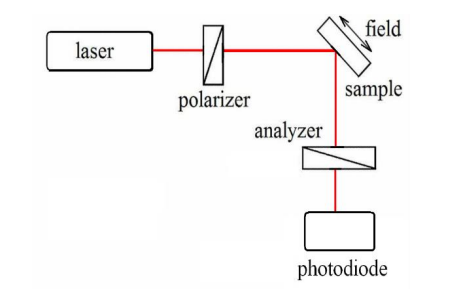
\includegraphics[width=0.6\textwidth]{fig/fig1.png}
    \caption{旋光的解释}\label{fig1}
\end{figure}
唯像的来看,线偏振光可以看成左旋和右旋偏振光的叠加。磁性介质中左旋、
右旋偏振光驱动介质当中电子作左旋和右旋圆周运动,由于磁场的存在,Lorenz
力对电子作用不同导致左旋、右旋光在传播时介质的响应,也就是介电常数不同 ,
因而给出磁光效应。假设一个线偏振的P光(偏振方向平行于入射面)从样品的
表面反射回来,如果样品是完全非磁的,反射回来的光依然是纯粹的P光;如果
样品带有铁磁性,反射光的偏振面相对于入射光的偏振面额外再转过了一个小的
角度,这个小角度称为克尔旋转角$\varPhi '$,因此反射光当中必然会掺杂进去S光的成
分。同时,由于介质对这两种模式的吸收率也不同,从而改变出射光的椭偏率$\varPhi ''$。
由于克尔旋转角$\varPhi '$和克尔椭偏率$\varPhi ''$都是磁化强度$M$的函
数。通过探测克尔旋转角或椭偏率的变化可以推测出磁化强度$M$的变化。

\section{实验内容}

\section{实验数据}

\section{误差分析}


\section{思考题}
\subsection*{如何获得椭偏率随磁场变化的曲线?}


\nocite{jiaocai}
\bibliography{ref}
\end{document}